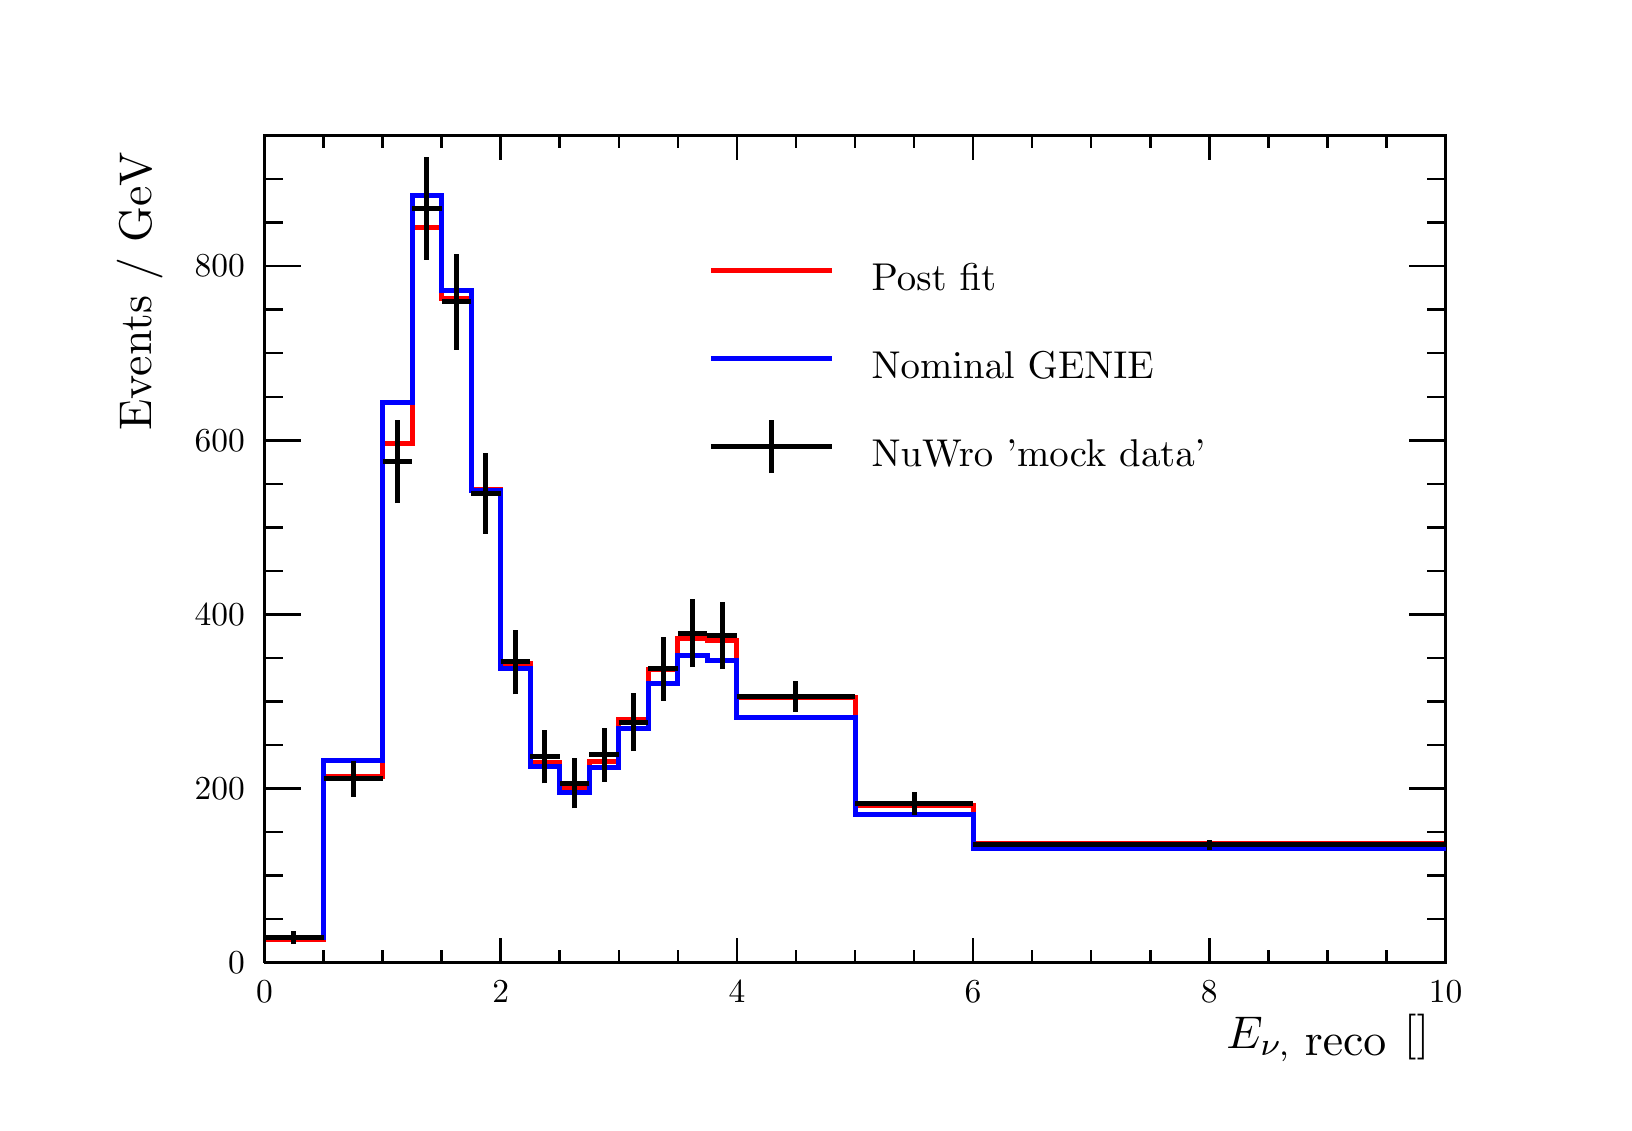
\begin{tikzpicture}
\pgfdeclareplotmark{cross} {
\pgfpathmoveto{\pgfpoint{-0.3\pgfplotmarksize}{\pgfplotmarksize}}
\pgfpathlineto{\pgfpoint{+0.3\pgfplotmarksize}{\pgfplotmarksize}}
\pgfpathlineto{\pgfpoint{+0.3\pgfplotmarksize}{0.3\pgfplotmarksize}}
\pgfpathlineto{\pgfpoint{+1\pgfplotmarksize}{0.3\pgfplotmarksize}}
\pgfpathlineto{\pgfpoint{+1\pgfplotmarksize}{-0.3\pgfplotmarksize}}
\pgfpathlineto{\pgfpoint{+0.3\pgfplotmarksize}{-0.3\pgfplotmarksize}}
\pgfpathlineto{\pgfpoint{+0.3\pgfplotmarksize}{-1.\pgfplotmarksize}}
\pgfpathlineto{\pgfpoint{-0.3\pgfplotmarksize}{-1.\pgfplotmarksize}}
\pgfpathlineto{\pgfpoint{-0.3\pgfplotmarksize}{-0.3\pgfplotmarksize}}
\pgfpathlineto{\pgfpoint{-1.\pgfplotmarksize}{-0.3\pgfplotmarksize}}
\pgfpathlineto{\pgfpoint{-1.\pgfplotmarksize}{0.3\pgfplotmarksize}}
\pgfpathlineto{\pgfpoint{-0.3\pgfplotmarksize}{0.3\pgfplotmarksize}}
\pgfpathclose
\pgfusepathqstroke
}
\pgfdeclareplotmark{cross*} {
\pgfpathmoveto{\pgfpoint{-0.3\pgfplotmarksize}{\pgfplotmarksize}}
\pgfpathlineto{\pgfpoint{+0.3\pgfplotmarksize}{\pgfplotmarksize}}
\pgfpathlineto{\pgfpoint{+0.3\pgfplotmarksize}{0.3\pgfplotmarksize}}
\pgfpathlineto{\pgfpoint{+1\pgfplotmarksize}{0.3\pgfplotmarksize}}
\pgfpathlineto{\pgfpoint{+1\pgfplotmarksize}{-0.3\pgfplotmarksize}}
\pgfpathlineto{\pgfpoint{+0.3\pgfplotmarksize}{-0.3\pgfplotmarksize}}
\pgfpathlineto{\pgfpoint{+0.3\pgfplotmarksize}{-1.\pgfplotmarksize}}
\pgfpathlineto{\pgfpoint{-0.3\pgfplotmarksize}{-1.\pgfplotmarksize}}
\pgfpathlineto{\pgfpoint{-0.3\pgfplotmarksize}{-0.3\pgfplotmarksize}}
\pgfpathlineto{\pgfpoint{-1.\pgfplotmarksize}{-0.3\pgfplotmarksize}}
\pgfpathlineto{\pgfpoint{-1.\pgfplotmarksize}{0.3\pgfplotmarksize}}
\pgfpathlineto{\pgfpoint{-0.3\pgfplotmarksize}{0.3\pgfplotmarksize}}
\pgfpathclose
\pgfusepathqfillstroke
}
\pgfdeclareplotmark{newstar} {
\pgfpathmoveto{\pgfqpoint{0pt}{\pgfplotmarksize}}
\pgfpathlineto{\pgfqpointpolar{44}{0.5\pgfplotmarksize}}
\pgfpathlineto{\pgfqpointpolar{18}{\pgfplotmarksize}}
\pgfpathlineto{\pgfqpointpolar{-20}{0.5\pgfplotmarksize}}
\pgfpathlineto{\pgfqpointpolar{-54}{\pgfplotmarksize}}
\pgfpathlineto{\pgfqpointpolar{-90}{0.5\pgfplotmarksize}}
\pgfpathlineto{\pgfqpointpolar{234}{\pgfplotmarksize}}
\pgfpathlineto{\pgfqpointpolar{198}{0.5\pgfplotmarksize}}
\pgfpathlineto{\pgfqpointpolar{162}{\pgfplotmarksize}}
\pgfpathlineto{\pgfqpointpolar{134}{0.5\pgfplotmarksize}}
\pgfpathclose
\pgfusepathqstroke
}
\pgfdeclareplotmark{newstar*} {
\pgfpathmoveto{\pgfqpoint{0pt}{\pgfplotmarksize}}
\pgfpathlineto{\pgfqpointpolar{44}{0.5\pgfplotmarksize}}
\pgfpathlineto{\pgfqpointpolar{18}{\pgfplotmarksize}}
\pgfpathlineto{\pgfqpointpolar{-20}{0.5\pgfplotmarksize}}
\pgfpathlineto{\pgfqpointpolar{-54}{\pgfplotmarksize}}
\pgfpathlineto{\pgfqpointpolar{-90}{0.5\pgfplotmarksize}}
\pgfpathlineto{\pgfqpointpolar{234}{\pgfplotmarksize}}
\pgfpathlineto{\pgfqpointpolar{198}{0.5\pgfplotmarksize}}
\pgfpathlineto{\pgfqpointpolar{162}{\pgfplotmarksize}}
\pgfpathlineto{\pgfqpointpolar{134}{0.5\pgfplotmarksize}}
\pgfpathclose
\pgfusepathqfillstroke
}
\definecolor{c}{rgb}{1,1,1};
\draw [color=c, fill=c] (0,0) rectangle (20,13.639);
\draw [color=c, fill=c] (3,1.77307) rectangle (18,12.2751);
\definecolor{c}{rgb}{0,0,0};
\draw [c,line width=0.9] (3,1.77307) -- (3,12.2751) -- (18,12.2751) -- (18,1.77307) -- (3,1.77307);
\definecolor{c}{rgb}{1,1,1};
\draw [color=c, fill=c] (3,1.77307) rectangle (18,12.2751);
\definecolor{c}{rgb}{0,0,0};
\draw [c,line width=0.9] (3,1.77307) -- (3,12.2751) -- (18,12.2751) -- (18,1.77307) -- (3,1.77307);
\definecolor{c}{rgb}{1,0,0};
\draw [c,line width=1.8] (3,2.07023) -- (3.75,2.07023) -- (3.75,4.13781) -- (4.5,4.13781) -- (4.5,8.35958) -- (4.875,8.35958) -- (4.875,11.111) -- (5.25,11.111) -- (5.25,10.2102) -- (5.625,10.2102) -- (5.625,7.78333) -- (6,7.78333) -- (6,5.56806) --
 (6.375,5.56806) -- (6.375,4.31399) -- (6.75,4.31399) -- (6.75,3.99747) -- (7.125,3.99747) -- (7.125,4.32564) -- (7.5,4.32564) -- (7.5,4.85745) -- (7.875,4.85745) -- (7.875,5.49486) -- (8.25,5.49486) -- (8.25,5.88922) -- (8.625,5.88922) --
 (8.625,5.8639) -- (9,5.8639) -- (9,5.14297) -- (10.5,5.14297) -- (10.5,3.77082) -- (12,3.77082) -- (12,3.28705) -- (18,3.28705);
\definecolor{c}{rgb}{0,0,0};
\draw [c,line width=0.9] (3,1.77307) -- (18,1.77307);
\draw [c,line width=0.9] (3,2.07994) -- (3,1.77307);
\draw [c,line width=0.9] (3.75,1.9265) -- (3.75,1.77307);
\draw [c,line width=0.9] (4.5,1.9265) -- (4.5,1.77307);
\draw [c,line width=0.9] (5.25,1.9265) -- (5.25,1.77307);
\draw [c,line width=0.9] (6,2.07994) -- (6,1.77307);
\draw [c,line width=0.9] (6.75,1.9265) -- (6.75,1.77307);
\draw [c,line width=0.9] (7.5,1.9265) -- (7.5,1.77307);
\draw [c,line width=0.9] (8.25,1.9265) -- (8.25,1.77307);
\draw [c,line width=0.9] (9,2.07994) -- (9,1.77307);
\draw [c,line width=0.9] (9.75,1.9265) -- (9.75,1.77307);
\draw [c,line width=0.9] (10.5,1.9265) -- (10.5,1.77307);
\draw [c,line width=0.9] (11.25,1.9265) -- (11.25,1.77307);
\draw [c,line width=0.9] (12,2.07994) -- (12,1.77307);
\draw [c,line width=0.9] (12.75,1.9265) -- (12.75,1.77307);
\draw [c,line width=0.9] (13.5,1.9265) -- (13.5,1.77307);
\draw [c,line width=0.9] (14.25,1.9265) -- (14.25,1.77307);
\draw [c,line width=0.9] (15,2.07994) -- (15,1.77307);
\draw [c,line width=0.9] (15.75,1.9265) -- (15.75,1.77307);
\draw [c,line width=0.9] (16.5,1.9265) -- (16.5,1.77307);
\draw [c,line width=0.9] (17.25,1.9265) -- (17.25,1.77307);
\draw [c,line width=0.9] (18,2.07994) -- (18,1.77307);
\draw [anchor=base] (3,1.26842) node[scale=1.20912, color=c, rotate=0]{0};
\draw [anchor=base] (6,1.26842) node[scale=1.20912, color=c, rotate=0]{2};
\draw [anchor=base] (9,1.26842) node[scale=1.20912, color=c, rotate=0]{4};
\draw [anchor=base] (12,1.26842) node[scale=1.20912, color=c, rotate=0]{6};
\draw [anchor=base] (15,1.26842) node[scale=1.20912, color=c, rotate=0]{8};
\draw [anchor=base] (18,1.26842) node[scale=1.20912, color=c, rotate=0]{10};
\draw [anchor= east] (18,0.812882) node[scale=1.65459, color=c, rotate=0]{$E_{\nu,~\textrm{reco}}$ [\si{\GeV}]};
\draw [c,line width=0.9] (3,12.2751) -- (18,12.2751);
\draw [c,line width=0.9] (3,11.9682) -- (3,12.2751);
\draw [c,line width=0.9] (3.75,12.1216) -- (3.75,12.2751);
\draw [c,line width=0.9] (4.5,12.1216) -- (4.5,12.2751);
\draw [c,line width=0.9] (5.25,12.1216) -- (5.25,12.2751);
\draw [c,line width=0.9] (6,11.9682) -- (6,12.2751);
\draw [c,line width=0.9] (6.75,12.1216) -- (6.75,12.2751);
\draw [c,line width=0.9] (7.5,12.1216) -- (7.5,12.2751);
\draw [c,line width=0.9] (8.25,12.1216) -- (8.25,12.2751);
\draw [c,line width=0.9] (9,11.9682) -- (9,12.2751);
\draw [c,line width=0.9] (9.75,12.1216) -- (9.75,12.2751);
\draw [c,line width=0.9] (10.5,12.1216) -- (10.5,12.2751);
\draw [c,line width=0.9] (11.25,12.1216) -- (11.25,12.2751);
\draw [c,line width=0.9] (12,11.9682) -- (12,12.2751);
\draw [c,line width=0.9] (12.75,12.1216) -- (12.75,12.2751);
\draw [c,line width=0.9] (13.5,12.1216) -- (13.5,12.2751);
\draw [c,line width=0.9] (14.25,12.1216) -- (14.25,12.2751);
\draw [c,line width=0.9] (15,11.9682) -- (15,12.2751);
\draw [c,line width=0.9] (15.75,12.1216) -- (15.75,12.2751);
\draw [c,line width=0.9] (16.5,12.1216) -- (16.5,12.2751);
\draw [c,line width=0.9] (17.25,12.1216) -- (17.25,12.2751);
\draw [c,line width=0.9] (18,11.9682) -- (18,12.2751);
\draw [c,line width=0.9] (3,1.77307) -- (3,12.2751);
\draw [c,line width=0.9] (3.462,1.77307) -- (3,1.77307);
\draw [c,line width=0.9] (3.231,2.3258) -- (3,2.3258);
\draw [c,line width=0.9] (3.231,2.87854) -- (3,2.87854);
\draw [c,line width=0.9] (3.231,3.43128) -- (3,3.43128);
\draw [c,line width=0.9] (3.462,3.98401) -- (3,3.98401);
\draw [c,line width=0.9] (3.231,4.53675) -- (3,4.53675);
\draw [c,line width=0.9] (3.231,5.08949) -- (3,5.08949);
\draw [c,line width=0.9] (3.231,5.64223) -- (3,5.64223);
\draw [c,line width=0.9] (3.462,6.19496) -- (3,6.19496);
\draw [c,line width=0.9] (3.231,6.7477) -- (3,6.7477);
\draw [c,line width=0.9] (3.231,7.30044) -- (3,7.30044);
\draw [c,line width=0.9] (3.231,7.85317) -- (3,7.85317);
\draw [c,line width=0.9] (3.462,8.40591) -- (3,8.40591);
\draw [c,line width=0.9] (3.231,8.95865) -- (3,8.95865);
\draw [c,line width=0.9] (3.231,9.51139) -- (3,9.51139);
\draw [c,line width=0.9] (3.231,10.0641) -- (3,10.0641);
\draw [c,line width=0.9] (3.462,10.6169) -- (3,10.6169);
\draw [c,line width=0.9] (3.462,10.6169) -- (3,10.6169);
\draw [c,line width=0.9] (3.231,11.1696) -- (3,11.1696);
\draw [c,line width=0.9] (3.231,11.7223) -- (3,11.7223);
\draw [c,line width=0.9] (3.231,12.2751) -- (3,12.2751);
\draw [anchor= east] (2.9,1.77307) node[scale=1.20912, color=c, rotate=0]{0};
\draw [anchor= east] (2.9,3.98401) node[scale=1.20912, color=c, rotate=0]{200};
\draw [anchor= east] (2.9,6.19496) node[scale=1.20912, color=c, rotate=0]{400};
\draw [anchor= east] (2.9,8.40591) node[scale=1.20912, color=c, rotate=0]{600};
\draw [anchor= east] (2.9,10.6169) node[scale=1.20912, color=c, rotate=0]{800};
\draw [anchor= east] (1.416,12.2751) node[scale=1.65459, color=c, rotate=90]{Events / GeV};
\draw [c,line width=0.9] (18,1.77307) -- (18,12.2751);
\draw [c,line width=0.9] (17.538,1.77307) -- (18,1.77307);
\draw [c,line width=0.9] (17.769,2.3258) -- (18,2.3258);
\draw [c,line width=0.9] (17.769,2.87854) -- (18,2.87854);
\draw [c,line width=0.9] (17.769,3.43128) -- (18,3.43128);
\draw [c,line width=0.9] (17.538,3.98401) -- (18,3.98401);
\draw [c,line width=0.9] (17.769,4.53675) -- (18,4.53675);
\draw [c,line width=0.9] (17.769,5.08949) -- (18,5.08949);
\draw [c,line width=0.9] (17.769,5.64223) -- (18,5.64223);
\draw [c,line width=0.9] (17.538,6.19496) -- (18,6.19496);
\draw [c,line width=0.9] (17.769,6.7477) -- (18,6.7477);
\draw [c,line width=0.9] (17.769,7.30044) -- (18,7.30044);
\draw [c,line width=0.9] (17.769,7.85317) -- (18,7.85317);
\draw [c,line width=0.9] (17.538,8.40591) -- (18,8.40591);
\draw [c,line width=0.9] (17.769,8.95865) -- (18,8.95865);
\draw [c,line width=0.9] (17.769,9.51139) -- (18,9.51139);
\draw [c,line width=0.9] (17.769,10.0641) -- (18,10.0641);
\draw [c,line width=0.9] (17.538,10.6169) -- (18,10.6169);
\draw [c,line width=0.9] (17.538,10.6169) -- (18,10.6169);
\draw [c,line width=0.9] (17.769,11.1696) -- (18,11.1696);
\draw [c,line width=0.9] (17.769,11.7223) -- (18,11.7223);
\draw [c,line width=0.9] (17.769,12.2751) -- (18,12.2751);
\definecolor{c}{rgb}{0,0,1};
\draw [c,line width=1.8] (3,2.09711) -- (3.75,2.09711) -- (3.75,4.34381) -- (4.5,4.34381) -- (4.5,8.87972) -- (4.875,8.87972) -- (4.875,11.5131) -- (5.25,11.5131) -- (5.25,10.3032) -- (5.625,10.3032) -- (5.625,7.76342) -- (6,7.76342) -- (6,5.51076)
 -- (6.375,5.51076) -- (6.375,4.25784) -- (6.75,4.25784) -- (6.75,3.93305) -- (7.125,3.93305) -- (7.125,4.24737) -- (7.5,4.24737) -- (7.5,4.74826) -- (7.875,4.74826) -- (7.875,5.31866) -- (8.25,5.31866) -- (8.25,5.67379) -- (8.625,5.67379) --
 (8.625,5.61364) -- (9,5.61364) -- (9,4.89062) -- (10.5,4.89062) -- (10.5,3.65793) -- (12,3.65793) -- (12,3.22384) -- (18,3.22384);
\definecolor{c}{rgb}{0,0,0};
\draw [c,line width=1.8] (3.375,2.00645) -- (3.375,2.09019);
\draw [c,line width=1.8] (3.375,2.09019) -- (3.375,2.17392);
\draw [c,line width=1.8] (3,2.09019) -- (3.375,2.09019);
\draw [c,line width=1.8] (3.375,2.09019) -- (3.75,2.09019);
\foreach \P in {(3.375,2.09019)}{\draw[mark options={color=c,fill=c},mark size=2.402402pt, line width=0.000000pt, mark=*,mark size=1pt] plot coordinates {\P};}
\draw [c,line width=1.8] (4.125,3.8786) -- (4.125,4.1057);
\draw [c,line width=1.8] (4.125,4.1057) -- (4.125,4.3328);
\draw [c,line width=1.8] (3.75,4.1057) -- (4.125,4.1057);
\draw [c,line width=1.8] (4.125,4.1057) -- (4.5,4.1057);
\foreach \P in {(4.125,4.1057)}{\draw[mark options={color=c,fill=c},mark size=2.402402pt, line width=0.000000pt, mark=*,mark size=1pt] plot coordinates {\P};}
\draw [c,line width=1.8] (4.6875,7.60769) -- (4.6875,8.13822);
\draw [c,line width=1.8] (4.6875,8.13822) -- (4.6875,8.66875);
\draw [c,line width=1.8] (4.5,8.13822) -- (4.6875,8.13822);
\draw [c,line width=1.8] (4.6875,8.13822) -- (4.875,8.13822);
\foreach \P in {(4.6875,8.13822)}{\draw[mark options={color=c,fill=c},mark size=2.402402pt, line width=0.000000pt, mark=*,mark size=1pt] plot coordinates {\P};}
\draw [c,line width=1.8] (5.0625,10.6986) -- (5.0625,11.3493);
\draw [c,line width=1.8] (5.0625,11.3493) -- (5.0625,12.0001);
\draw [c,line width=1.8] (4.875,11.3493) -- (5.0625,11.3493);
\draw [c,line width=1.8] (5.0625,11.3493) -- (5.25,11.3493);
\foreach \P in {(5.0625,11.3493)}{\draw[mark options={color=c,fill=c},mark size=2.402402pt, line width=0.000000pt, mark=*,mark size=1pt] plot coordinates {\P};}
\draw [c,line width=1.8] (5.4375,9.5563) -- (5.4375,10.1655);
\draw [c,line width=1.8] (5.4375,10.1655) -- (5.4375,10.7747);
\draw [c,line width=1.8] (5.25,10.1655) -- (5.4375,10.1655);
\draw [c,line width=1.8] (5.4375,10.1655) -- (5.625,10.1655);
\foreach \P in {(5.4375,10.1655)}{\draw[mark options={color=c,fill=c},mark size=2.402402pt, line width=0.000000pt, mark=*,mark size=1pt] plot coordinates {\P};}
\draw [c,line width=1.8] (5.8125,7.21777) -- (5.8125,7.73105);
\draw [c,line width=1.8] (5.8125,7.73105) -- (5.8125,8.24433);
\draw [c,line width=1.8] (5.625,7.73105) -- (5.8125,7.73105);
\draw [c,line width=1.8] (5.8125,7.73105) -- (6,7.73105);
\foreach \P in {(5.8125,7.73105)}{\draw[mark options={color=c,fill=c},mark size=2.402402pt, line width=0.000000pt, mark=*,mark size=1pt] plot coordinates {\P};}
\draw [c,line width=1.8] (6.1875,5.18023) -- (6.1875,5.59112);
\draw [c,line width=1.8] (6.1875,5.59112) -- (6.1875,6.00201);
\draw [c,line width=1.8] (6,5.59112) -- (6.1875,5.59112);
\draw [c,line width=1.8] (6.1875,5.59112) -- (6.375,5.59112);
\foreach \P in {(6.1875,5.59112)}{\draw[mark options={color=c,fill=c},mark size=2.402402pt, line width=0.000000pt, mark=*,mark size=1pt] plot coordinates {\P};}
\draw [c,line width=1.8] (6.5625,4.04934) -- (6.5625,4.38948);
\draw [c,line width=1.8] (6.5625,4.38948) -- (6.5625,4.72962);
\draw [c,line width=1.8] (6.375,4.38948) -- (6.5625,4.38948);
\draw [c,line width=1.8] (6.5625,4.38948) -- (6.75,4.38948);
\foreach \P in {(6.5625,4.38948)}{\draw[mark options={color=c,fill=c},mark size=2.402402pt, line width=0.000000pt, mark=*,mark size=1pt] plot coordinates {\P};}
\draw [c,line width=1.8] (6.9375,3.73057) -- (6.9375,4.04771);
\draw [c,line width=1.8] (6.9375,4.04771) -- (6.9375,4.36486);
\draw [c,line width=1.8] (6.75,4.04771) -- (6.9375,4.04771);
\draw [c,line width=1.8] (6.9375,4.04771) -- (7.125,4.04771);
\foreach \P in {(6.9375,4.04771)}{\draw[mark options={color=c,fill=c},mark size=2.402402pt, line width=0.000000pt, mark=*,mark size=1pt] plot coordinates {\P};}
\draw [c,line width=1.8] (7.3125,4.06831) -- (7.3125,4.40977);
\draw [c,line width=1.8] (7.3125,4.40977) -- (7.3125,4.75122);
\draw [c,line width=1.8] (7.125,4.40977) -- (7.3125,4.40977);
\draw [c,line width=1.8] (7.3125,4.40977) -- (7.5,4.40977);
\foreach \P in {(7.3125,4.40977)}{\draw[mark options={color=c,fill=c},mark size=2.402402pt, line width=0.000000pt, mark=*,mark size=1pt] plot coordinates {\P};}
\draw [c,line width=1.8] (7.6875,4.45737) -- (7.6875,4.82472);
\draw [c,line width=1.8] (7.6875,4.82472) -- (7.6875,5.19206);
\draw [c,line width=1.8] (7.5,4.82472) -- (7.6875,4.82472);
\draw [c,line width=1.8] (7.6875,4.82472) -- (7.875,4.82472);
\foreach \P in {(7.6875,4.82472)}{\draw[mark options={color=c,fill=c},mark size=2.402402pt, line width=0.000000pt, mark=*,mark size=1pt] plot coordinates {\P};}
\draw [c,line width=1.8] (8.0625,5.09759) -- (8.0625,5.50375);
\draw [c,line width=1.8] (8.0625,5.50375) -- (8.0625,5.90992);
\draw [c,line width=1.8] (7.875,5.50375) -- (8.0625,5.50375);
\draw [c,line width=1.8] (8.0625,5.50375) -- (8.25,5.50375);
\foreach \P in {(8.0625,5.50375)}{\draw[mark options={color=c,fill=c},mark size=2.402402pt, line width=0.000000pt, mark=*,mark size=1pt] plot coordinates {\P};}
\draw [c,line width=1.8] (8.4375,5.52401) -- (8.4375,5.95398);
\draw [c,line width=1.8] (8.4375,5.95398) -- (8.4375,6.38395);
\draw [c,line width=1.8] (8.25,5.95398) -- (8.4375,5.95398);
\draw [c,line width=1.8] (8.4375,5.95398) -- (8.625,5.95398);
\foreach \P in {(8.4375,5.95398)}{\draw[mark options={color=c,fill=c},mark size=2.402402pt, line width=0.000000pt, mark=*,mark size=1pt] plot coordinates {\P};}
\draw [c,line width=1.8] (8.8125,5.49983) -- (8.8125,5.92849);
\draw [c,line width=1.8] (8.8125,5.92849) -- (8.8125,6.35715);
\draw [c,line width=1.8] (8.625,5.92849) -- (8.8125,5.92849);
\draw [c,line width=1.8] (8.8125,5.92849) -- (9,5.92849);
\foreach \P in {(8.8125,5.92849)}{\draw[mark options={color=c,fill=c},mark size=2.402402pt, line width=0.000000pt, mark=*,mark size=1pt] plot coordinates {\P};}
\draw [c,line width=1.8] (9.75,4.9601) -- (9.75,5.15341);
\draw [c,line width=1.8] (9.75,5.15341) -- (9.75,5.34672);
\draw [c,line width=1.8] (9,5.15341) -- (9.75,5.15341);
\draw [c,line width=1.8] (9.75,5.15341) -- (10.5,5.15341);
\foreach \P in {(9.75,5.15341)}{\draw[mark options={color=c,fill=c},mark size=2.402402pt, line width=0.000000pt, mark=*,mark size=1pt] plot coordinates {\P};}
\draw [c,line width=1.8] (11.25,3.64295) -- (11.25,3.79236);
\draw [c,line width=1.8] (11.25,3.79236) -- (11.25,3.94177);
\draw [c,line width=1.8] (10.5,3.79236) -- (11.25,3.79236);
\draw [c,line width=1.8] (11.25,3.79236) -- (12,3.79236);
\foreach \P in {(11.25,3.79236)}{\draw[mark options={color=c,fill=c},mark size=2.402402pt, line width=0.000000pt, mark=*,mark size=1pt] plot coordinates {\P};}
\draw [c,line width=1.8] (15,3.20243) -- (15,3.26667);
\draw [c,line width=1.8] (15,3.26667) -- (15,3.33092);
\draw [c,line width=1.8] (12,3.26667) -- (15,3.26667);
\draw [c,line width=1.8] (15,3.26667) -- (18,3.26667);
\foreach \P in {(15,3.26667)}{\draw[mark options={color=c,fill=c},mark size=2.402402pt, line width=0.000000pt, mark=*,mark size=1pt] plot coordinates {\P};}
\definecolor{c}{rgb}{1,1,1};
\draw [color=c, fill=c] (2,12.8206) rectangle (18,13.5708);
\definecolor{c}{rgb}{0,0,0};
%\draw (10,13.1957) node[scale=1.40004, color=c, rotate=0]{$\nu_{\mu} FHC postfit: \delta = 1.57, \chi^{2} = 2.33$};
\definecolor{c}{rgb}{1,1,1};
\draw [color=c, fill=c] (8.33811,7.76504) rectangle (17.1347,11.1175);
\definecolor{c}{rgb}{0,0,0};
\draw [anchor=base west] (10.5372,10.3073) node[scale=1.40004, color=c, rotate=0]{Post fit};
\definecolor{c}{rgb}{1,0,0};
\draw [c,line width=1.8] (8.66798,10.5587) -- (10.2074,10.5587);
\definecolor{c}{rgb}{0,0,0};
\draw [anchor=base west] (10.5372,9.18983) node[scale=1.40004, color=c, rotate=0]{Nominal GENIE};
\definecolor{c}{rgb}{0,0,1};
\draw [c,line width=1.8] (8.66798,9.44126) -- (10.2074,9.44126);
\definecolor{c}{rgb}{0,0,0};
\draw [anchor=base west] (10.5372,8.07235) node[scale=1.40004, color=c, rotate=0]{NuWro 'mock data'};
\draw [c,line width=1.8] (8.66798,8.32378) -- (10.2074,8.32378);
\draw [c,line width=1.8] (9.43768,7.98854) -- (9.43768,8.65903);
\end{tikzpicture}
